% !TEX root = ../thesis.tex
% створюємо розділ
\chapter{Огляд}
\label{chap:distributedcomputation}

Має сенс більш детально розглянути проблеми, з якими наша нація може з деякою
імовірністю зіштовхнутися у майбутньому.

\pagestyle{plain}

    \section{Загальний огляд та класифікація}\label{sec:general}
        Питання, які Україні доведеться вирішувати через деякий час, природньо поділяються на два класи:

        \begin{enumerate}
            \item Загальнолюдські проблеми
            \item Специфічно українські проблеми
        \end{enumerate}
        
        Спробуємо дати класифікації підтипів, що мають місце у цих класах. 

        Загальнолюдські проблеми можна поділити на:

        \begin{enumerate}
            \item Економічні:
            \begin{itemize}
                \item Зміна структури зайнятості
                \item Зростання нерівності у доходах
            \end{itemize}

            \item Екологічні:
            \begin{itemize}
                \item Зменшення біорізноманіття
                \item Зміна клімату
                \item Забруднення довкілля
            \end{itemize}

            \item Соціальні:
            \begin{itemize}
                \item Неоднорідна освітня модернізація
                \item Масштабна урбанізація
                \item Гендерна нерівність
                \item Зростання політичного популізму
            \end{itemize}
        \end{enumerate}

        Поділ специфічних проблем для України може бути таким:

        \begin{enumerate}
            \item Економічні:
            \begin{itemize}
                \item Ресурсозалежність
                \item Відсутність іноваційності
            \end{itemize}

            \item Екологічні:
            \begin{itemize}
                \item Забруднення, зокрема гідроресурсів
                \item Наслідки Чорнобилю та проблема зберігання ядерних відходів
                \item Вичерпання лісоресурсу
            \end{itemize}

            \item Соціальні:
            \begin{itemize}
                \item Старіння населення та еміграція
                \item Застаріла освіта
                \item Війна з Російською Федерацією
                \item Внутрішня нестабільність і надмірна централізованість
            \end{itemize}
        \end{enumerate}

        Наведену класифікацію можна наочно відобразити у вигляді mind map --- ієрархічного
        способу подання інформації \cite{hopper2015practicing}. Згенерована за
        допомогою програми SimpleMind Lite \cite{simplemind} така mind map наведена на рисунку \ref{fig:mindmap}.

        \begin{figure}[!htp]
            \centering
            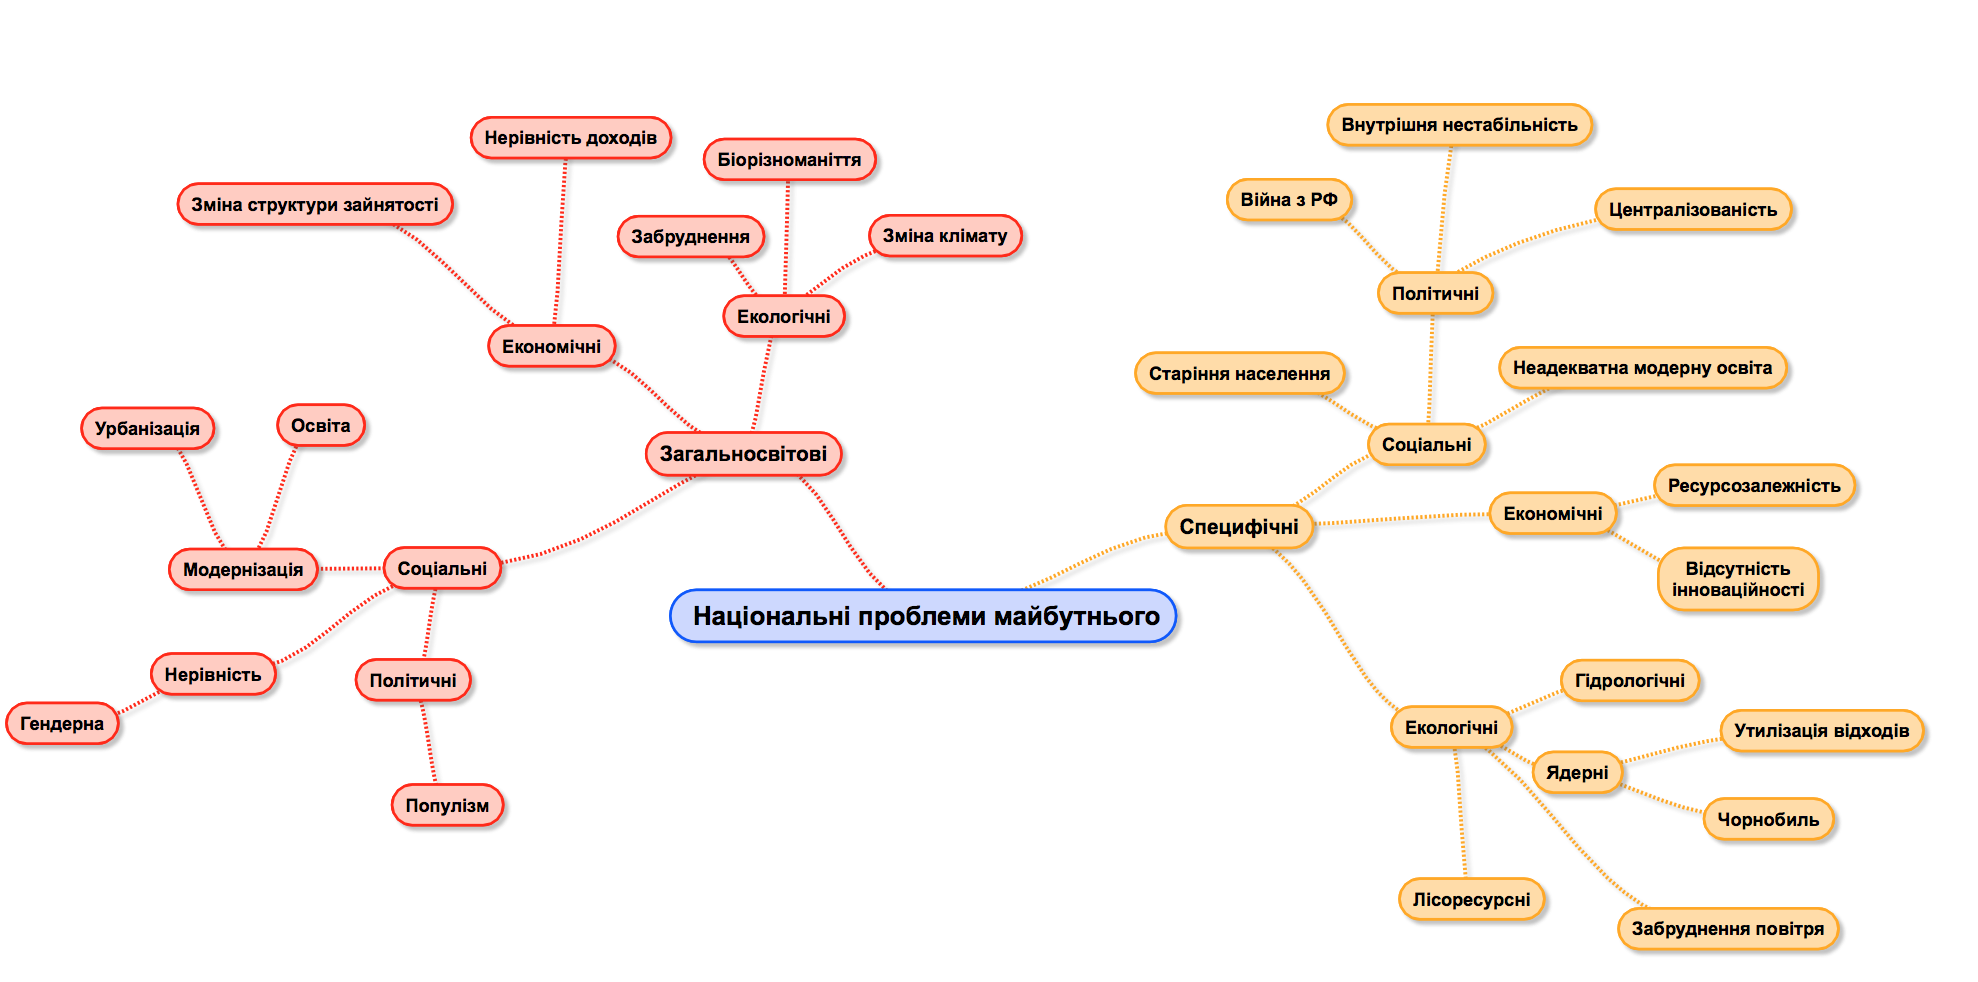
\includegraphics[scale = 0.5]{PNG/mindmap.png}
            \caption{Mind map}
            \label{fig:mindmap}
        \end{figure}

    \section{Загальнолюдські проблеми}\label{sec:world}